\documentclass[12pt]{article}

% Any percent sign marks a comment to the end of the line

% Every latex document starts with a documentclass declaration like this
% The option dvips allows for graphics, 12pt is the font size, and article
%   is the style




% array/table
\usepackage{array}
\usepackage{multirow}

% figure
\usepackage[pdftex]{graphicx}
\usepackage{epsfig}
\usepackage[hang]{subfigure}
\usepackage[small,bf]{caption}
\usepackage{amsmath}
\usepackage{enumitem}
\usepackage{tabularx}
\usepackage{ctable}


\usepackage{authblk}
\renewcommand\Authands{ and }

%clickable ref
\usepackage[backref,pagebackref,naturalnames=true,colorlinks]{hyperref}



\setlength{\oddsidemargin}{0.25in}
\setlength{\textwidth}{6.5in}
\setlength{\topmargin}{0in}
\setlength{\textheight}{8.5in}



%----------------------------------------------------------------------------------------
%	DOCUMENT INFORMATION
%----------------------------------------------------------------------------------------

\title{EG01-EG23 Transition: Cyclus Results}


\author[1]{B. Mouginot\thanks{\href{mailto:mouginot@wisc.edu}{mouginot@wisc.edu}}}
\author[1]{P.P.H. Wilson \thanks{\href{mailto:paul.wilson@wisc.edu}{paul.wilson@wisc.edu}}}
\author[1]{R. Carlsen \thanks{\href{mailto:rcarlsen@wisc.edu}{rcarlsen@wisc.edu}}}
\affil[1]{University of Wisconsin--Madison, Department of Engineering Physics, CNERG group}


\date{\today}

\setlength{\parindent}{0em}
\setlength{\parskip}{0.7em}

\begin{document}
\maketitle

\section{Intro/specification}
The U.S. Department of Energy (DOE) Fuel Cycle Option (FCO) started a study 
campaign to assess the future of the U.S. nuclear fleet. After considering 
equilibrium scenario, called Evaluation Group (EG), the Doe has been interested in 
assessing the transition  from the current fuel cycle to some of those 
equilibrium scenarios, pre-emptively studied.\\
The goal of this study is to model the transition from a once-through light
water reactor (LWR) fuel cycle (i.e. EG01) to a sodium fast reactor (SFR) full
recycle case (i.e. EG23).\\
This calculation has been done after the one performed by the three established 
fuel cycle simulator DYMON (ANL) \cite{dymond}, VISION (INL) \cite{vision}, 
and ORION (ORNL \cite{orion}. The goal was to illustrated the capabilities of the 
Cyclus simulator, an agent based fuel cycle simulator developed at University of 
Wisconsin-Madison. \\
 The LWR and SFR deployments were selected to accomplish three primary goals:

\begin{itemize}
    \item Follow the 1\% annual electricity production curve (Figure \ref{fig:nrg}).
    \item Minimize the amount of sitting separated plutonium.
    \item Transition as quickly as possible given the other goals.
\end{itemize}

\section{Scenario Description}

By default, Cyclus facilities exhibit greedy behavior, they request and
process as much material as they can given their inventory capacities and
process limits.  As Cyclus does not yet include direct support for on-demand
processing, some special accommodations were made to maintain the desired low
inventory of separated Pu.  In order to address this in parts, a series of two
simulations were run:

\begin{itemize}

    \item \textbf{Case 1}: A simulation with fuel fabrication deployments
        matching capacity for SFR fresh fuel demand over time, but with
        unrestricted, greedy spent fuel separations.

    \item \textbf{Case 2}: A simulation with separations throughput changing
        over time. Results from the first simulation were used to calculate
        the required separations deployments over time in order to approximate
        on-demand separations.

\end{itemize}

Scenario details for cases 1 and 2 are identical except for those noted in
Section \ref{sec:case2}.

Scenario details are based on previous work done by R. Carlsen, which
can be found there (TODO: where?).  From this study, the configuration and
deployment schedule of the separation facilities for LWR used fuel have been
taken. The rest of the study has been adapted from it, to match B. Feng DYMOND
analysis \cite{B.Feng_calculation}.

The deployment schedule (Figure \ref{fig:deploy}) has not been calculated
using Cyclus, it has been taken from B. Feng calculation and implemented in
Cyclus (with some approximation which will be detailed further in the
document).

\begin{figure}[h!]
    \centering
    \subfigure[Deployment schedule\label{fig:deploy}]     {\epsfig{figure=img/CapacityStarted,width=0.48\textwidth}}
    \subfigure[Electricity produced\label{fig:nrg}]		{\epsfig{figure=img/ElectricityGenerated,width=0.48\textwidth}}
    \caption{
        Deployment schedule and corresponding electricity produced by the
        different reactors where R1(blue): existing LWR, R2(green): new
        builded LWR, R3(red): high SFR, R4(purple): low
        SFR.\label{fig:deployment}
    }
\end{figure}

The following subsections describe the configuration of the primary facility
types (i.e. Cyclus prototypes) used in this analysis.

\subsection{Reactors}

After the LWR to SFR transition is completed, new SFR reactors are deployed
with a lower breeding ratio in order to prevent unbounded buildup of
plutonium. The properties of the different reactors cores used for the
simulation have been summarized in Table \ref{tab:reactor}.

\begin{table}[h!]
    \centering
    \begin{tabularx}{350pt}{lXXX}
    \hline
    Core Properties       &	LWR     &	SFR 1   &	SFR 2     \\
    \hline
    Rated Power, [MWe]    &	1000		&	400     &	400       \\
    Thermal Efficiency    &	N.A.$^1$	&	0.4     &	0.4       \\
    Capacity Factor       &	0.90		&	0.90		&	0.90      \\
    Number of batches     &	6       &	5       &	3         \\
    Cycle length, [month] &	9       &	13      &	18        \\
    Core Inventory, [tHM] &	14.784*6&	7.524*5	&	11.466*3  \\
    \hline
    \end{tabularx}
    \caption{Reactor core properties.}
    \label{tab:reactor}
    \footnotesize{$^1$ I don't have this number, but as a recipe reactor is used, it is not required.}
\end{table}

Because of the 1-month timestep of Cyclus, a few liberties have been taken
with the batch quantity and cycle length parameters in order to match as
closely as possible important invariants such as fuel residence time, burnup,
and discharge rates \cite{REF-F.Bo}.  For the SFR 1 facility type, the cycle
length is supposed to be 5.44 y (for discharge burnup of 37.62 GWd/t), 5.41 y
has been used (5 * 13 months). For SFR 2, 4.5y has been used (3 * 18 months)
where 4.44 was expected.  With Cyclus' 1-month time step, the burnup invariant
can be easly calculated as:

\begin{equation}
  \Delta BU = \frac{P_{th} \times \Delta t}{M_{r}},
\end{equation}

\noindent where $P_{th}$ is the thermal power of the reactor, $M_{r}$ its mass
in heavy metal, $\Delta BU$ the burnup achievable precision and $\Delta t$ the
time step size.  In this simulation the $\Delta BU$ are for the SFR 1 \& 2
respectively: $0.73$ and $0.79~GWd/t$.  This does not affect the composition
of the discharge fuel as the reactor model used for this analysis does not
perform a burnup evolution calculation.  Only the mass of discharged fuel is
affected with a relative error of :

\begin{equation}
  \frac{\Delta M}{M} = \frac{\Delta BU}{BU}.
\end{equation}

All LWR reactors use enriched uranium fuel. The SFR used MOX fuel with
different plutonium enrichments. The input/output fuel recipes are summarized
in Table \ref{tab:reactor_fuel} taken from \cite{B.Feng_calculation}.

\begin{table}[h!]
    \centering
    \begin{tabular}{lllll}
    \hline
    \multicolumn{2}{c}{Reactor}			&	LWR [$\%w$]	&	SFR fuel 1  [$\%w$]	&	SFR fuel 2  [$\%w$] 	\\
    \hline
    \multirow{3}{*} {In recipe}	&	235U	&	95.8			&	0				&	0				\\
    &	238U	&	4.2			&	92.36			&	91.466			\\
    &	Pu		&	0			&	7.64				&	8.534			\\
    \hline
    \multirow{5}{*} {Out recipe}&	235U	&	0.8			&	0				&	0				\\
    &	238U/U	&	92.68		&	85.99			&	86.025			\\
    &	Pu		&	1.2			&	9.02				&	9.596			\\
    &	MA		&	0.11			&	0.13				&	0.107			\\
    &	FP		&	5.21			&	4.86				&	4.272			\\
    \hline
    \end{tabular}

    \caption{
        Input/Output Fuel composition recipe for the different reactors. Note that
        for the SFR reactor fuel no isotopic distinctions have been made and U in
        SFR should be considered depleted uranium in the input recipes, the
        uranium isotopic changes in the output recipes have not been investigated
        in this work.
    }

    \label{tab:reactor_fuel}
\end{table}

\subsection{Cooling/Storage}

After irradiation, all fuel is cooled for 84 months before becoming available
for reprocessing.  The Cycacore Storage facility allows defining a minimum
residence time for each incoming material.  In order to simplify
differentiating between material in cooling and material available for
reprocessing, 2 storage facilities are used in series providing this explicit
separation. One dedicated to cooling, with a residence time of 84 months, and
one dedicated to storage until reprocessing with no minimum residence time
providing data for the "UNF waiting for reprocessing" and the "Resource in
storage" output data columns respectively.  Notable are subtle differences in
what these two storage facilities' data represent and their exact semantic
meaning in the analysis spreadsheet.

\subsection{Separation}

The LWR fuel separation is handled by three identical separation facilities,
two deployed in 2030 and one in 2040. The SFR separation facilities have a
very large separation capacity, in the first case, we have tried to throttle
the separation rate indirectly using the gradual fuel fabrication capacity
growth. Full fabrication facilities stop requesting separated plutonium
leading to eventual halting of spent fuel separations.

\begin{table}[h!]
    \centering
    \begin{tabular}{lllll}
    \hline
    Separation Properties	&	LWR		&	SFR 1/2	\\
    \hline
    Throughput [tML]		&	83.3333	&	5000		\\
    feed buffer [tML]		&	107.537	&	5000		\\
    Pu output  [tML]		&	Unlimited	&	5000		\\
    Pu separation efficiency	&	0.99		&	0.99		\\
    Recycled Uranium [tML]	&	Unlimited	&	Unlimited	\\
    U separation efficiency	&	0.99		&	0.99		\\
    Waste [tML]			&	Unlimited	&	Unlimited	\\
    \hline
    \end{tabular}
    \caption{Separation facilities core properties. }
    \label{tab:separation_1}
\end{table}

\subsection{Fuel Fabrication}

The UOX fuel fabrication is handled by one enrichment facility, the properties
of this enrichment facilities are summarized in Table \ref{tab:enrich_1}.

\begin{table}[h!]
    \centering
    \begin{tabular}{lllll}
    \hline
    Enrichment Properties	&	UOX		\\
    \hline
    Throughput [tML]		&	Unlimited	\\
    swu capacity [tML]		&	1e97		\\
    tails assay  			&	0.0025	\\
    Initial feed [tML]		&	Unlimited	\\
    \hline
    \end{tabular}
    \caption{Enrichment facilities properties. }
    \label{tab:enrich_1}
\end{table}

The SFR fuel fabrication facilities are supposed to be deployed as a rate of 1
for every 10 SFRs.  As the fuel composition and annual flux slightly change
between SFR 1 and 2, the specifications between fabrication are also slightly
different. The details of all fuel fabrication facility characteristics are
summarized in Table \ref{tab:fuelfab_1}.

\begin{table}[h!]
    \centering
    \begin{tabular}{lllll}
    \hline
    Fuel Fab Properties	&	SFR 1	&	SFR 2	\\
    \hline
    Throughput [tML]	&	75.240	&	76.440	\\
    depleted buffer [tML]	&	69.492	&	69.912	\\
    Pu buffer  [tML]		&	5.748	&	5.856	\\
    \hline
    \end{tabular}
    \caption{Fuel fabrication facilities properties.}
    \label{tab:fuelfab_1}
\end{table}

\section{On-demand Separations: Case 2 Differences}
\label{sec:case2}

The only difference with the Case 1 scenario is the way in
which reprocessing capacity is handled over time.  Modeling on-demand
separations requires deploying separations facilities according to plutonium
requirements for SFR fuel fabrication.  These Pu requirements were determined
from the Case 1 results. While the calculated deployment schedule does not
follow plutonium usage exactly, it is a good rough aproximation. 

For this calculation, all fuel are reprocessed by only one type of
reprocessing facility (i.e. one Cyclus prototype). The fuel input preferences
have been set to 3 for all irradiated UOX fuel, 2 for higher breeding ratio
SFR spent fuel, and 3 for the lower breeding ratio SFR spent fuel (a higher
number indicates a higher preference).  The characteristics of each of the
reprocessing facilities used in Case 2 are summarized in Table
\ref{tab:fuelfab_2}.

\begin{table}[h!]
    \centering
    \begin{tabular}{ll}
    \hline
    Separation Properties	&	All Fuel	\\
    \hline
    Throughput [tML]		&	60		\\
    feed buffer [tML]		&	66		\\
    Pu output  [tML]		&	6		\\
    Pu separation efficiency	&	0.99		\\
    Recycled Uranium [tML]	&	Unlimited	\\
    U separation efficiency	&	0.99		\\
    Waste [tML]			&	Unlimited	\\
    \hline
    \end{tabular}
    \caption{Separation facilities core properties.}
    \label{tab:fuelfab_2}
\end{table}

\section{Results}

\subsection{Case 1: Greedy Separations}

All fuel loading metrics (Figure \ref{fig:RessourceUsed}) are the same or very
close to DYMOND simulation results. There are some observable fluctuations on
the annual fuel loading and the SWU requirements which are consistent with the
synchronized refueling cycles of the initially deployed reactors.  There are
various simple ways to stagger refueling cycles for smoother data that were
not pursued in this analysis.

\begin{figure}[h!]
    \centering
    \subfigure[Ressources Mined]			{\epsfig{figure=img/RessourceMined,width=0.48\textwidth}}
    \subfigure[SWU Requirement]			{\epsfig{figure=img/SWURequierment,width=0.48\textwidth}}
    \subfigure[Annual Fuel Loading Rate]	{\epsfig{figure=img/AnnualFuelLoading,width=0.48\textwidth}}
    \caption{Ressources production and fuel loading.\label{fig:RessourceUsed} }
\end{figure}

The generated power and the deployment schedule (Figure \ref{})  match
perfectly with results from the DYMOND simulations. The sudden drop in 2210 is
due to a lack of deployment data after 2210 due to limitations of the DYMOND
code which was used as the source for deployments.

\begin{figure}[h!]
    \centering
    \subfigure[Deployment schedule]	{\epsfig{figure=img/CapacityStarted,width=0.48\textwidth}}
    \subfigure[Electricity produced ]		{\epsfig{figure=img/ElectricityGenerated,width=0.48\textwidth}}
    \caption{Deployment schedule and corresponding
    electricity produced by the different reactors
    where R1(blue): existing LWR, R2(green): new
    builded LWR, R3(red): high SFR, R4(purple): low
    SFR.\label{fig:deployment_bis} }
\end{figure}

The other curves also appear as expected. The annual reprocessing rate
corresponds directly to the deployments. Spent UOX reprocessing starts in 2010
with 2000 MTHM/yr with another 1000 MTHM/yr added in 2030.  This reprocessing
rate (UOX1 + UOX2) continues until the end of the production of used UOX (i.e.
when all LWRs are decommissioned).

\begin{figure}[h!]
    \centering
    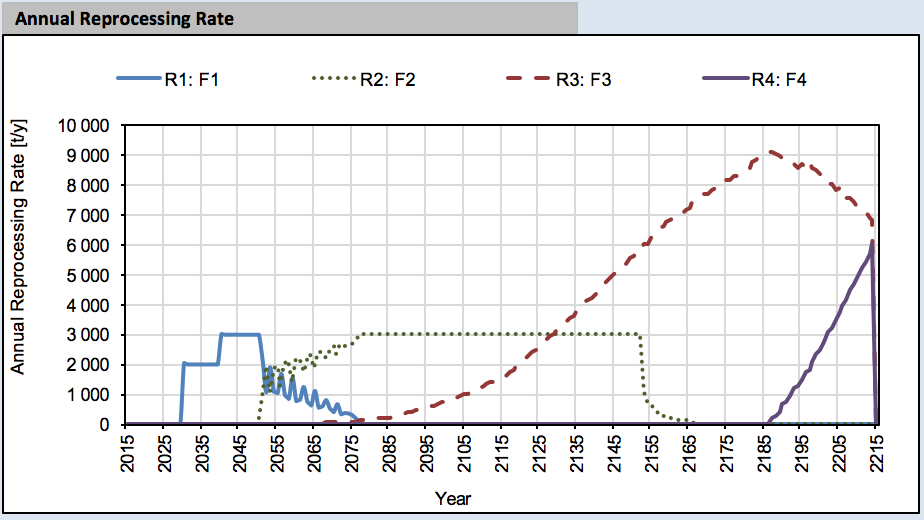
\includegraphics[width=0.62\textwidth]	{img/AnnualReprocessingRate_1}
    \caption{Annual Reprocessing Rate.}
    \label{fig:reprocessing_1}
\end{figure}


MOX spent fuel production by the 2 different SFR types roughly follows the
loading of fresh fuel.  Because the reprocessing facilities are greedy,
reprocessing all used fuel available, there is no SFR spent fuel in storage
because it is directly reprocessed after cooling.

\begin{figure}[h!]
    \centering
    \subfigure[Used Fuel in Cooling]		{\epsfig{figure=img/usedFuelInCooling,width=0.48\textwidth}}
    \subfigure[Fuel waiting for reprocessing]	{\epsfig{figure=img/UNFWaitingReprocessing_1,width=0.48\textwidth}}
    \caption{Used fuel in cooling and reprocessing.\label{fig:cool_reprocc} }
\end{figure}

As almost all SFR spent fuel are directly reprocessed after cooling, spent
fuel in storage stops increasing when all the UOX fuel has been reprocessed.

\begin{figure}[h!]
    \centering
    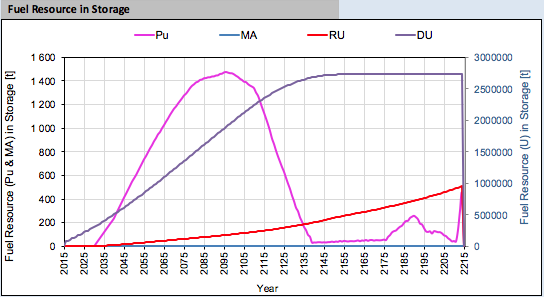
\includegraphics[width=0.62\textwidth]{img/FuelInStorage_1}
    \caption{Storage Fuel composition.}
    \label{fig:storagecompo_1}
\end{figure}

It appears that the capacity of the SFR fuel reprocessing is not enough to
reprocess the full inventory of MOX fuel until 2155. This explains the
appearance of MOX fuel in storage waiting for reprocessing. With the
replacement of higher breeding ratio SFRs with lower breeding ratio reactors
the MOX spent fuel generation rate decreases sufficiently for reprocessing to
"catch-up".

As shown in the Figures \ref{fig:FC_Z} and \ref{fig:WR_Z}, the quantity of
plutonium in storage follows the variation in the amount of MOX1 fuel in
storage.

\begin{figure}[h!]
    \centering
    \subfigure[Storage Fuel composition (zoomed)\label{fig:FC_Z}]		{\epsfig{figure=img/FuelInStorage_1_zoom,width=0.48\textwidth}}
    \subfigure[Fuel waiting for reprocessing (zoomed)\label{fig:WR_Z}]	{\epsfig{figure=img/UNFWaitingReprocessing_1_zoom,width=0.48\textwidth}}
    \caption{Plutonium in storage.\label{fig:FC_WR_zoom} }
\end{figure}

\subsection{Case 2: On-demand Separations}

The only differences in the results between the two cases can be seen in the
behavior of the reprocessed fuel --- namely in the UNF fuel waiting for
reprocessing and in the composition of material in storage.

\begin{figure}[h!]
    \centering
    \subfigure[Annual Reprocessing Rate]			{\epsfig{figure=img/AnnualReprocessingRate_2,width=0.48\textwidth}}
    \subfigure[Fuel waiting for reprocessing]			{\epsfig{figure=img/UNFWaitingReprocessing_2,width=0.48\textwidth}}
    \subfigure[Storage Fuel composition]	{\epsfig{figure=img/FuelInStorage_2,width=0.48\textwidth}}
    \caption{Ressources production and fuel loading.\label{fig:ARR_FWR_SFC_2} }
\end{figure}

Indeed, as seen in Figure 8a., the reprocessing follows the plutonium need of
the SFR fuel fabrication. The UOX spent fuel only contains about only 1\% of
plutonium while SFR spent fuel contains about 10\%, which explains the sudden
decrease in the amount of fuel reprocessed around year 2110.  When switching
to the higher plutonium content spent fuel, the separations facilities are
able to produce an equivalent amount of fissile Pu while processing much less
material from their spent fuel input inventories.

Because of both the reprocessing priority and "on-demand" separations
deployment, we observe more fuel waiting for reprocessing with a quick drop
starting around year 2090 as stored up plutonium is used in the first wave of
SFR deployments replacing aging LWRs.  We can also observe some of SFR fuel
waiting for reprocessing, which decrease slowly, showing a well designed SFR
deployment schedule that reaches an comfortable equilibrium generating
plutonium at the same rate it is being recycled.

\section{Summary}

This study has shown the capability of Cyclus to properly simulate the EG01 to
EG23 fuel cycle transition.  The main observable differences are in the
reprocessing and the storage of the used fuel, where the meaning of desired
output data (e.g. "Fuel Resource in Storage", "UNF waiting for reprocessing",
etc.) were ambiguous.  Much of the inability of Cyclus to reproduce results
from other simulators exactly can likely be attributed to this factor.

Despite Cyclus is not able now to handle exact on-demand behavior, it is
possible to deploy the different facilities with limited capacities to
"follow" material demand to mimicking an on-demand type of behavior, as shown
in Case 2.  We can also observe some small differences in the pattern of fuel
loading (and almost all the reactor fuel metrics), this comes from the way
batches are modeled discretely in Cyclus where in DYMOND all entities are
material flows are managed in a more incremental, continuous way.

%----------------------------------------------------------------------------------------
%	BIBLIOGRAPHY
%----------------------------------------------------------------------------------------

\bibliographystyle{unsrt}

\bibliography{}

%----------------------------------------------------------------------------------------

\end{document}
